\centerline{\bf \Huge Теория чисел. МТФ+Теорема Эйлера.}
\title{Теория чисел. МТФ+Теорема Эйлера.}

\textit{Малая теорема Ферма. Пусть $a$ $-$ некоторое число, которое не делится на простое число $p$. Тогда верно, что $a^{p-1} \equiv 1 \ (mod \ p)$}.

\par

\textit{Лемма.}  Для любого простого числа $p$ и целого числа $k$, не кратного $p$, числа $1, 2, 3, \dots , p-1$ и числа $k\cdot 1,  k \cdot 2, \dots ,  k \cdot (p-1)$  при делении на $p$ в остатке дают те же самые числа возможно, записанные в некотором другом порядке.

\par 

\textit{Доказательство леммы:}\\
Понятно, что для доказательства леммы достаточно доказать, что во втором наборе чисел все остатки при делении на $p$ разные. Пусть $a, b \in \{$1, 2,$ \dots , p - 1\}$ и $a \neq b$. (Пояснение для тех, кого пугает такая запись. Это означает, что $a$ и $b$ это какие-то разные числа от $1$ до $p-1$). Предположим так получилось, что числа $ak$ и $bk$ дают одинаковые остатки при делении на $p$. Тогда $ak \equiv bk \ (mod \ p)$. Но мы знаем, что $(k, p) = 1$, а значит можем поделить обе части на $k$. Тогда получаем, что $a \equiv b \ (mod \ p)$, чего быть не может, так как $a$ и $b$ это разные числа от $1$ до $p$. Лемма доказана. Теперь перейдем к доказательству самой теоремы Ферма.

\textit{Доказательство МТФ:}\\
Поскольку (в силу доказанной леммы) остатки от деления на $p$ чисел $a, a\cdot1, a\cdot2, \dots, a\cdot(p-1)$ это c точностью до перестановки числа $1, 2, \dots, p-1$, то тогда равны и произведения этих чисел. То есть  $a\cdot 2a \cdot 3a \cdot \ldots \cdot a(p-1) \equiv 1 \cdot 2 \cdot \ldots \cdot (p-1) \ (mod \ p)$. Последнее соотношение можно сократить на $(p - 1)!$, поскольку все сомножители являются числами, взаимно простыми с числом $p$.\\
В результате получаем требуемое утверждение $a^{p-1} \equiv 1 \ (mod \ p).$

\textit{Комбинаторное доказательство через раскраски:}\\
На рисунке изображены все $32$ способа раскраски в два цвета круга, который разделен на $5$ равных секторов. Среди них выделяются два способа $-$ когда весь круг синий и когда он весь красный. А остальные разбиты на $6$ групп по  раскрасок, получающихся одна из другой поворотом.

\begin{figure}[h] 
    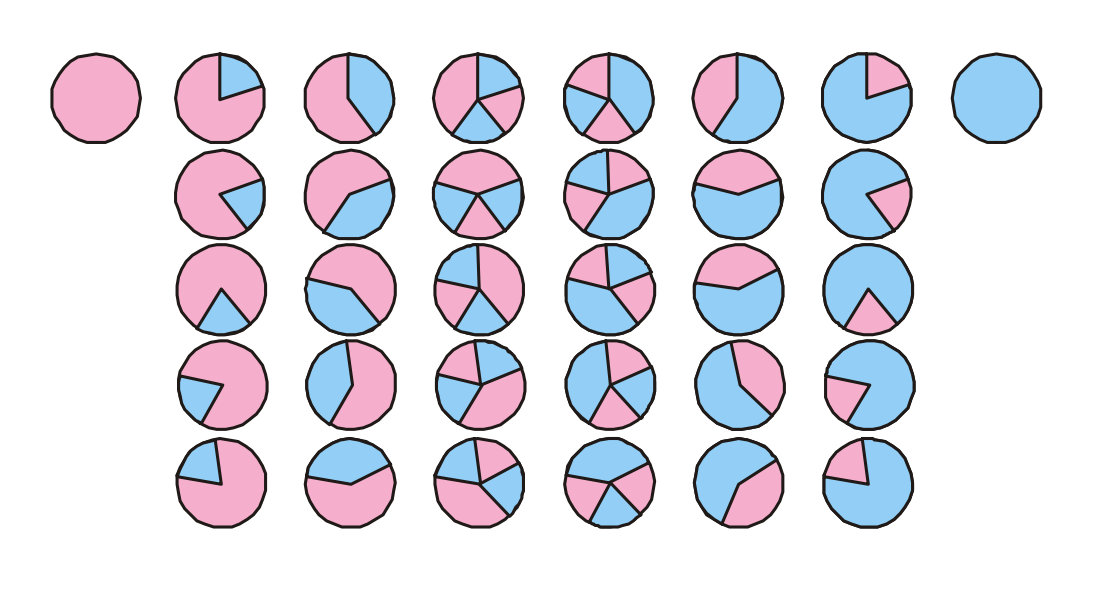
\includegraphics[scale=0.25]{Лососи_Весна_2023/FermaKMB.png}
\end{figure}

\newpage

\hspace{3mm}

\textit{Задача.} Сколькими способами можно раскрасить $a$ разными красками круг, разбитый на $p$ одинаковых секторов, где $p \ -$ простое число? (Каждый сектор окрашивается одной краской; не обязательно использовать все краски; две раскраски, совпадающие при повороте круга, считаются одинаковыми.)

\par

\textit{Решение задачи:}\\
Сперва посчитаем сколько одноцветных раскрасок. Очевидно их столько же сколько различных красок, то есть $a$ штук. Всего раскрасок $a^{p}$ штук (так для каждого из $p$ секторов есть $a$ вариантов его покрасить). Значит разноцветных раскрасок ровно $a^{p} - a$ штук. Но вот из любой разноцветной раскраски поворотами можно получить $p$ разных раскрасок (считая и саму эту раскраску: она получается поворотом на 0°). Но по задаче раскраски переходящие друг в друга поворотами считаются одинаковыми, а значит разных с точки зрения условиия раскрасок $a + \dfrac{a^p - a }{p}$. Поскольку количество способов не бывает дробным, число $a^{p} - a$ обязано делиться на $p$. МТФ доказана!\\

\textbf{\Large{Пару примеров применения МТФ в задачах.}}\\

\textit{Пример 1.} Докажите, что $3^{3000}-1$ делится на $1001$.

\textit{Решение:} Разложим 1001 на простые множители $1001 = 7\cdot 11 \cdot 13$. Применим малую теорему Ферма по модулю $7, 11, 13$. Получим, что 
$3^6 \equiv 1 \ (mod \ 7)$, $3^{10} \equiv 1 \ (mod \ 11)$, $3^{12} \equiv 1 \ (mod \ 13)$. 
Осталось заметить, что 
$3000 = 6 \cdot 500 = 10 \cdot 300 = 12 \cdot 250$, 
то есть
$3^{3000} \equiv 1 \ (mod \ 7), 3^{3000} \equiv 1 \ (mod \ 11), 3^{3000} \equiv 1 \ (mod \ 13)$, 
а значит $3^{3000}-1$ делится на $1001$.\\

\textit{Пример 2.} Пусть $N$ чётное число, не делящееся на $10$. Найдите предпоследнюю цифру числа $N^{20}$.

\textit{Решение:} Из условия следует, что $N$ не делится на $5$. Тогда по малой теореме Ферма имеет, что 
$N^{4} \equiv 1 \ (mod \ 5)$. Поэтому $N^{20} - 1 = (N^{4} - 1)(N^{16}+N^{12}+N^{8}+N^{4}+1)$ делится на $25$. Поскольку $N$ чётно, то оно оканчивается либо на $26$ либо на $76$. Но число, оканчивающееся на $26$ не делится на $4$.
Стало быть $N$ оканчивается на $76$ и предпоследняя цифра равна $7$.

\newpage

\hspace{3mm}

\textbf{\Large{От Ферма к Эйлеру.}} Начнём с определения очень важной функции. 

\textit{Определение.} Функция Эйлера $\varphi (n) \ - $ это функция, которая считает количество чисел от $1$ до $n$, которые взаимно просты с $n$. 

\par 

Некоторые важные свойства функции Эйлера:

1) $\varphi (p) = p-1$, где $p$ простое число.

2) $\varphi (p^{n}) = p^{n}- p^{n-1}$ 

3) $\varphi (mn) = \varphi (m)\varphi (n)$, где $m$ и $n$ взаимно простые числа.

4) Пусть $n = p_1^{\alpha_1}p_2^{\alpha_2} \dots p_k^{\alpha_k}$ - это называется каноническое разложение числа. Иначе говоря каждое число можно представить в виде произведени степеней простых чисел. Например, $36 = 2^2 \cdot 3^2$ или $720 = 2^4 \cdot 3^2 \cdot 5^1$. Тогда функцию Эйлера от числа $n$ можно вычислить следующим образом: 
$\boldsymbol{\varphi (n) = \varphi (p_1^{\alpha_1}) \varphi (p_2^{\alpha_2}) \dots \varphi (p_k^{\alpha_k})}$. То есть достаточно вычислить функцию Эйлера от каждой степени, а потом их перемножить. \\
\textit{Пример вычисления:}
$\varphi (1575) = \varphi (3^2 \cdot 5^2 \cdot 7^1) = \varphi (3^2) \cdot \varphi (5^2) \cdot \varphi (7^1) = 6 \cdot 20 \cdot 6 = 720$

По сути единственная сложность в вычислении функции Эйлера это разложить число на степени простых. Теперь перейдем к основному утверждению!

\textit{Теорема Эйлера. Пусть $a$ и $m$ взаимно просты. Тогда $a^{\varphi (m)} \equiv 1 \ (mod \ m)$}, где $\varphi (m)$ это функция Эйлера.

\par 

\textit{Доказательство:}

Пусть $x_1, x_2, \dots, x_{\varphi (m)} \ - $ все различные числа, меньшие $m$ и взаимно простые с ним. Умножим все эти числа на какое-нибудь $a$, которое тоже взаимно просто с $m$(действуем по аналогии с доказательством МТФ). Получим новый набор $ax_1, ax_2, \dots, ax_{\varphi (m)}$. Давайте покажем, что первый набор чисел и второй совпадают с точки зрения остатков при делении на $m$. Для этого достаточно показать, что во втором наборе все остатки разные(то что они взаимно просты с $m$ очевидно). Точно так же, как и с МТФ возьмём два различных числа и предположим, что они дают одинаковые остатки при делении на $m$. То есть $ax_1 \equiv ax_2 \ (mod \ m)$ (для того чтобы не заморачиваться с индексами взяли $x_1$ и $x_2$). Сокращаем на $a$ и получаем противоречие. Далее после того как доказали, что эти два набора равны, как остатки при делении на $m$, то проделываем такой же заключительный шаг, как и в МТФ. Перемножаем числа внутри наборов и приравниваем. Предлагаю его  проделать вам самим и завершить тем самым доказательство теоремы!

\textbf{Задачи для самопроверки:}

\problem{1} Докажите, используя малую теорему Ферма, что $a^{p^2} \equiv a \ (mod \ p)$, где $p -$ простое число.

\problem{2} Найдите остатки от деления на 83 чисел:

а) $10^{82}$

б) $10^{165}$

в) $10^{100!}$

\problem{3} Докажите, что $13^{160} - 1$ делится на $187$

\problem{4} Докажите, что $300^{480} - 1$ делится на $1001$